% Fig. R2-1: sealed quantitative result
\begin{figure*}[t]
  \centering
  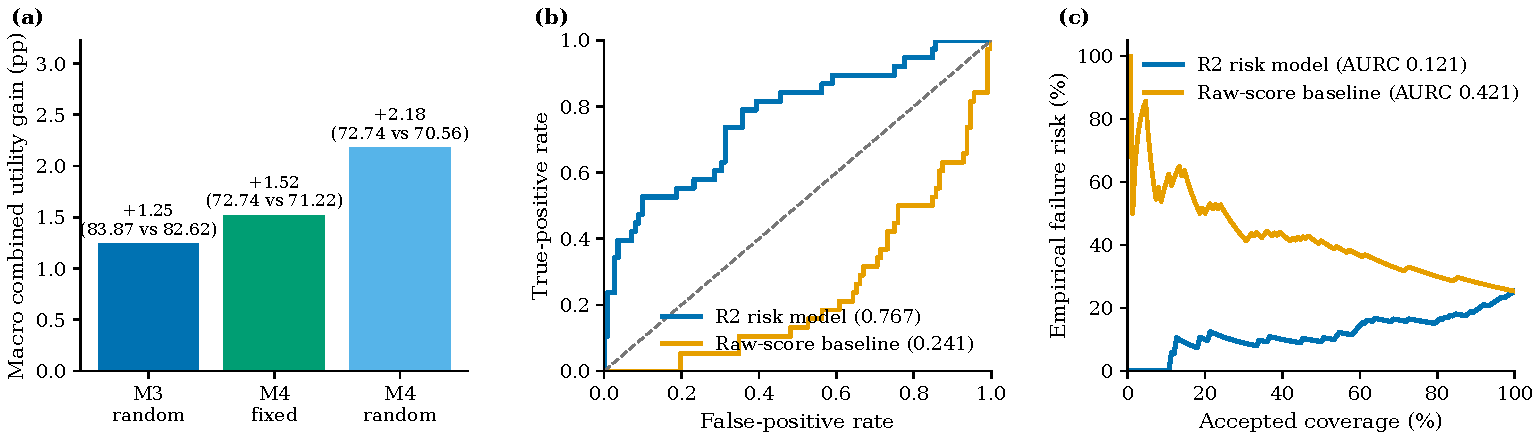
\includegraphics[width=0.98\textwidth]{reports/r2/figures/r2_sealed_metrics.pdf}
  \caption{One-time sealed validation on 150 recorded Photoneo targets from 139 physical tracks disjoint from the score-calibration tracks. (a) Macro combined pose-utility gain for M3-R2 over exact-budget matched random and M4-R2 over fixed slot 2 and uniform-random view selection. (b--c) Failure ROC and risk--coverage for the deployable M6-R2 model versus the raw FoundationPose-score baseline. This is same-sensor, calibration-track-disjoint evidence, not an unseen-sensor result or simulation.}
  \label{fig:r2-sealed-metrics}
\end{figure*}

% Fig. M5-R3-1: failed sealed gate diagnostics
\begin{figure*}[t]
  \centering
  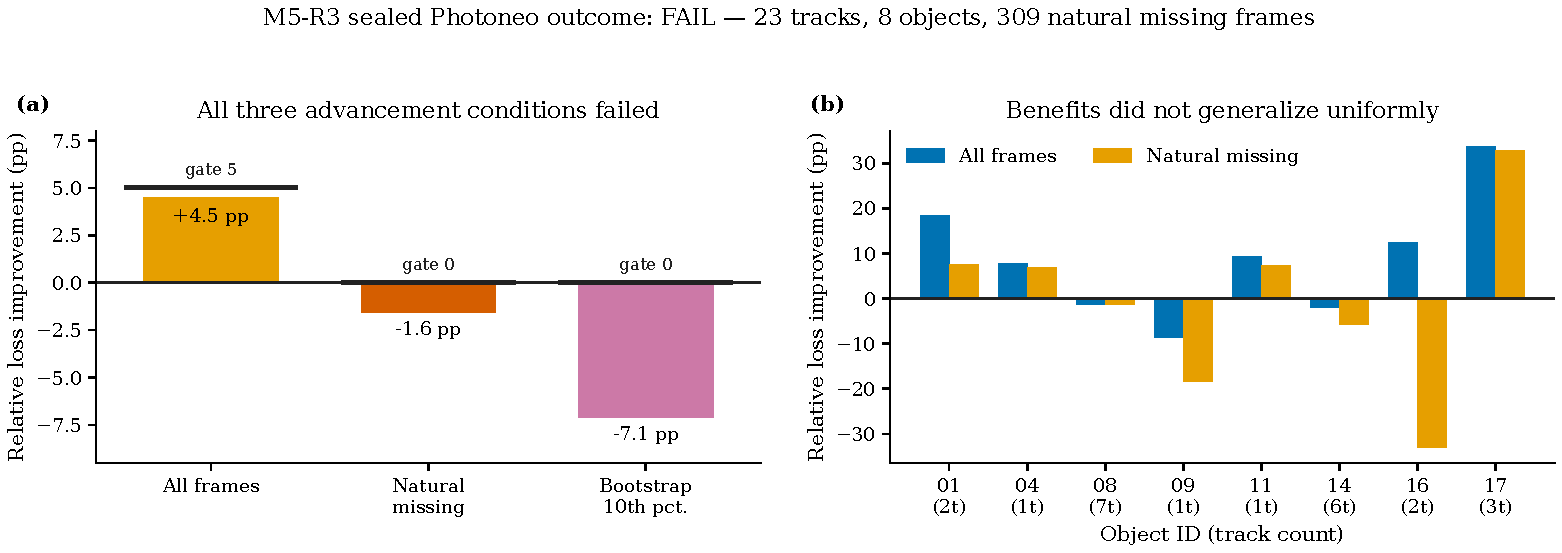
\includegraphics[width=0.98\textwidth]{reports/r2/figures/m5_r3_sealed_metrics.pdf}
  \caption{One-time M5-R3 sealed replay of a RealSense-developed static quotient medoid on 23 naturally incomplete Photoneo tracks (8 objects, 309 missing frames) disjoint from all prior R1/R2 Photoneo group tracks. Replay uses a nominal 20 Hz clock and oracle association. The method missed every frozen advancement condition: all-frame loss improvement was $+4.5\%$ (required $\geq5\%$), natural-missing improvement was $-1.6\%$ (required $\geq0$), and the hierarchical-bootstrap 10th percentile was $-7.1\%$ (required $\geq0$). This is a negative static-world result, not unseen-object, hardware-timestamp, moving-object, or deployable-association evidence.}
  \label{fig:m5-r3-sealed-metrics}
\end{figure*}

% Fig. M5-R3-2: natural-missing content examples
\begin{figure*}[t]
  \centering
  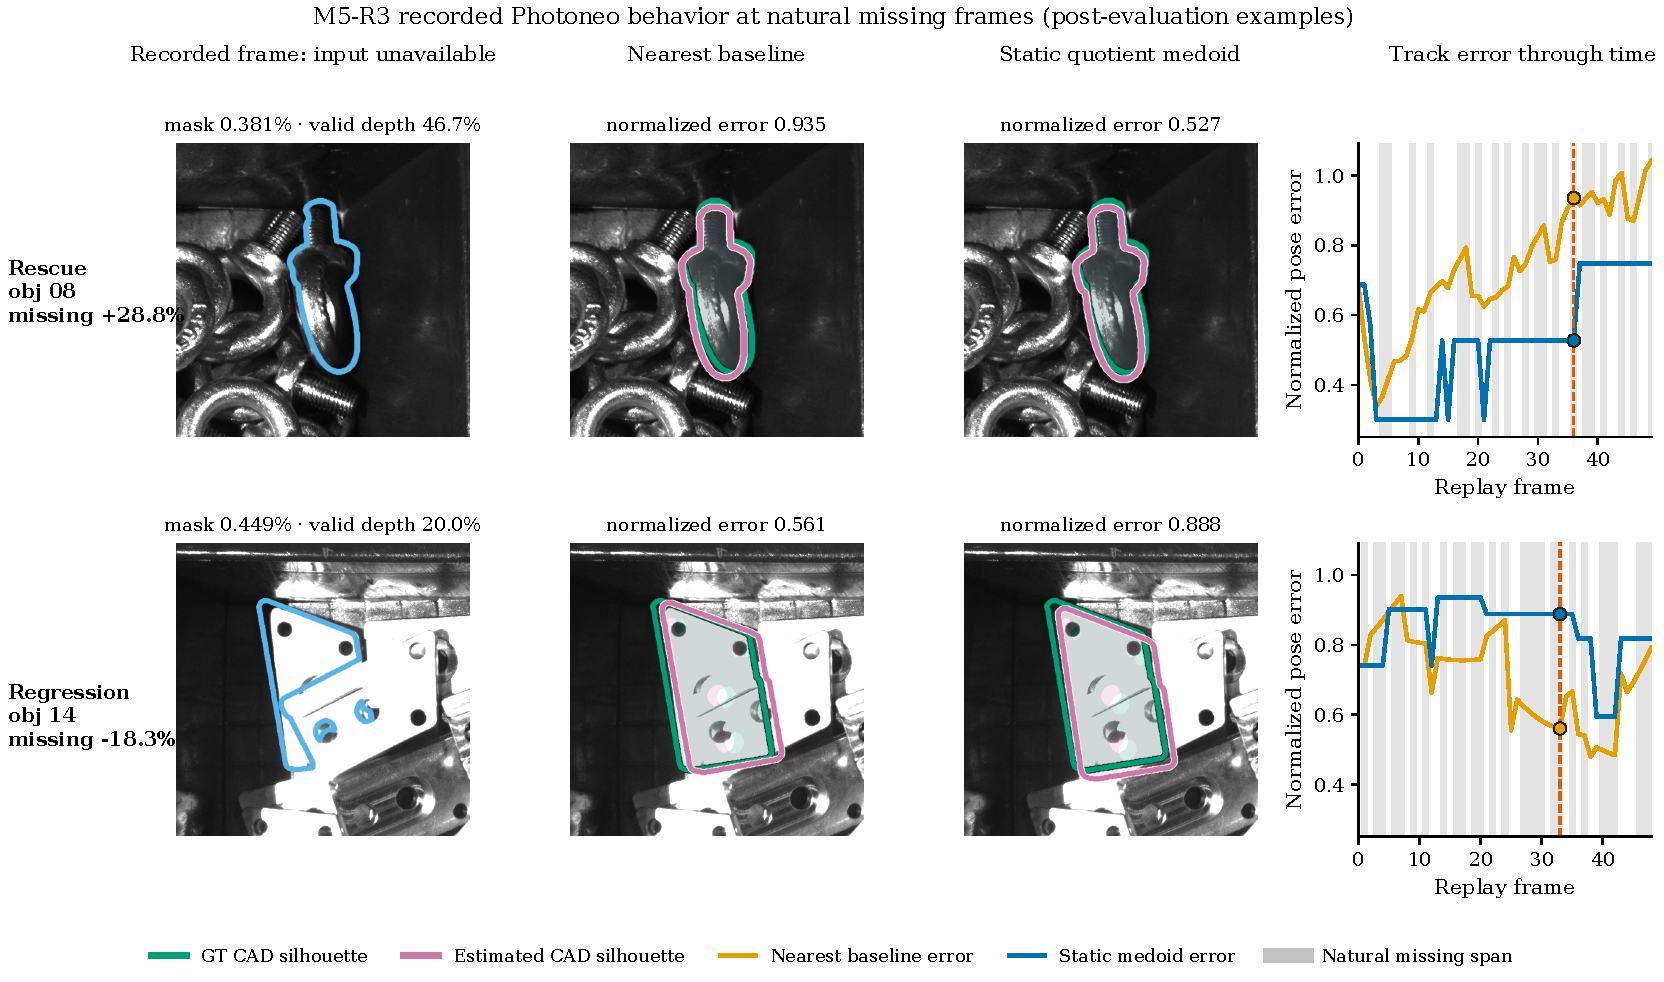
\includegraphics[width=0.98\textwidth]{reports/r2/figures/m5_r3_content_examples.pdf}
  \caption{Recorded Photoneo behavior at natural input-missing frames for the frozen nearest baseline and RealSense-developed M5-R3 static quotient medoid, using nominal timing and oracle association. Green and magenta contours are ground-truth and estimated CAD silhouettes with dark/light halos. Gray time-series spans denote naturally unavailable inputs; the dashed line marks the displayed frame, and both rows share the same error scale. Post-evaluation visualization first restricts to tracks with at least 10 missing frames and baseline missing-frame loss at most 2.0, then selects the greatest rescue and regression within that subset. These examples do not change the failed sealed result and are not simulator output, human visual acceptance, or deployable-association evidence.}
  \label{fig:m5-r3-content}
\end{figure*}

% Fig. R2-2: real-observation before/after examples
\begin{figure*}[t]
  \centering
  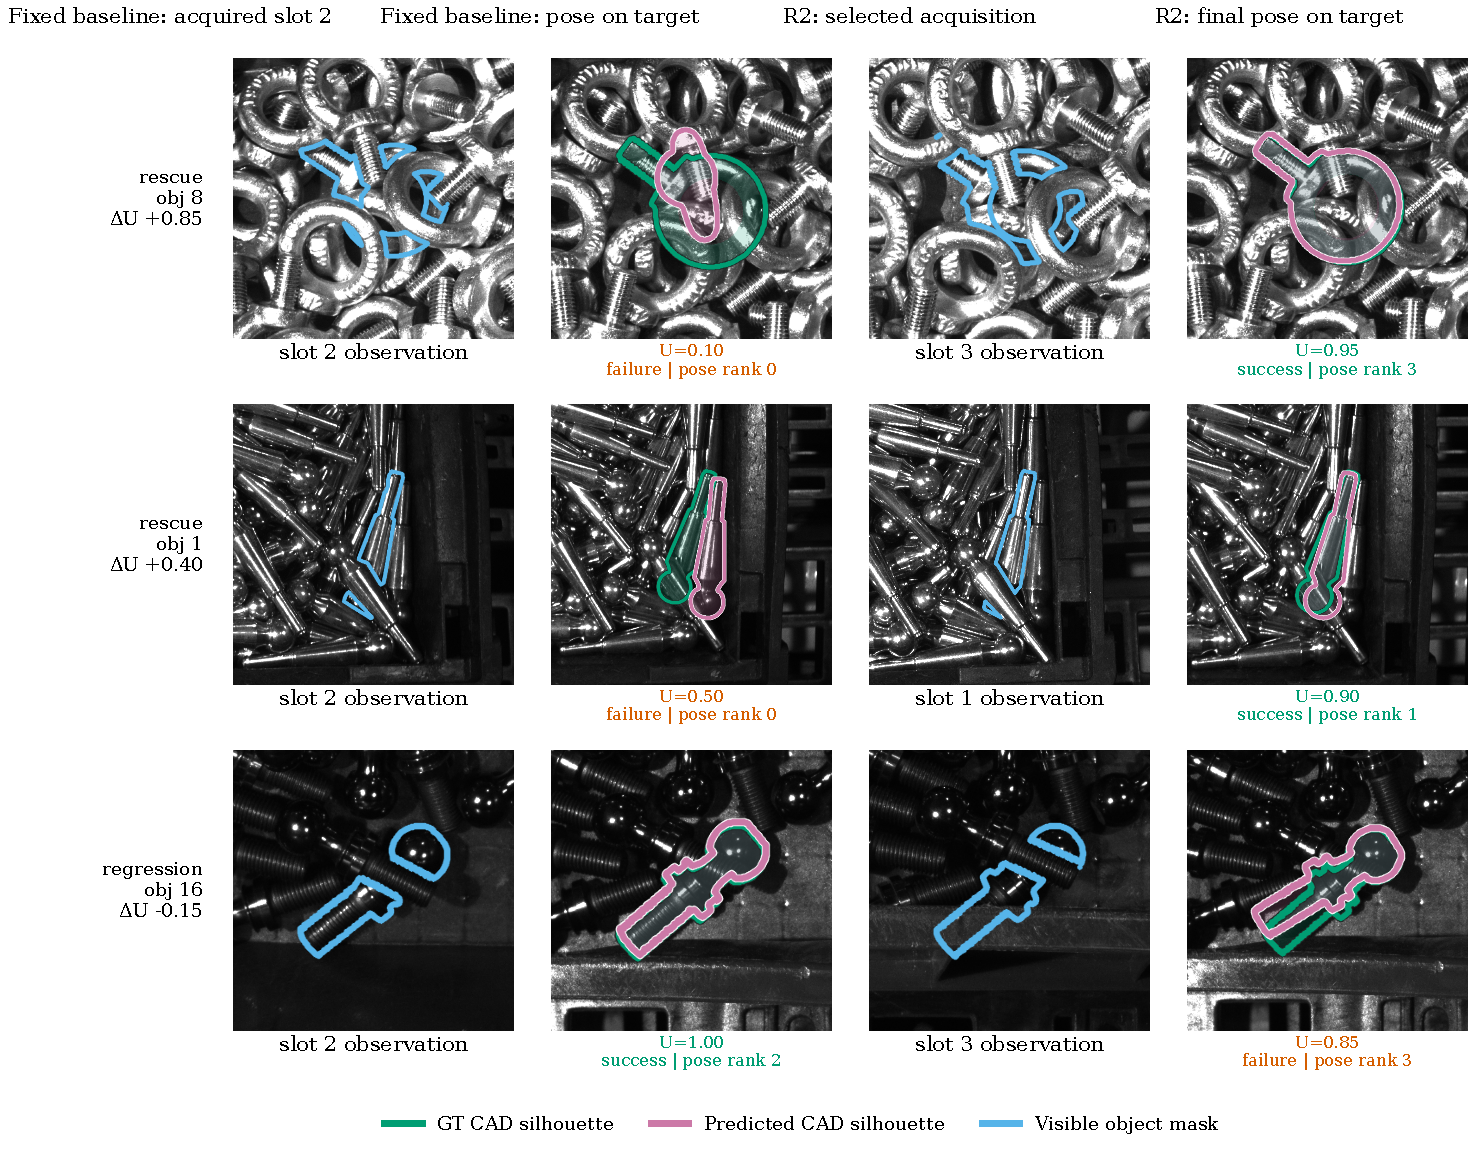
\includegraphics[width=0.98\textwidth]{reports/r2/figures/r2_m4_content_examples.pdf}
  \caption{Recorded Photoneo examples comparing the fixed-slot-2 baseline with frozen M4-R2 selection. Green and magenta contours are ground-truth and predicted CAD silhouettes projected into the target camera; contrasting dark/light halos preserve their distinction in grayscale. Success is the sealed joint criterion (normalized MSSD $\leq 0.10$ and MSPD $\leq 10r$, where $r$ is image width divided by 640), not human visual judgment. Rows are selected deterministically after evaluation for visualization only: two largest cross-object rescues and the largest regression.}
  \label{fig:r2-m4-content}
\end{figure*}

% Fig. R2-3: deployable risk examples
\begin{figure*}[t]
  \centering
  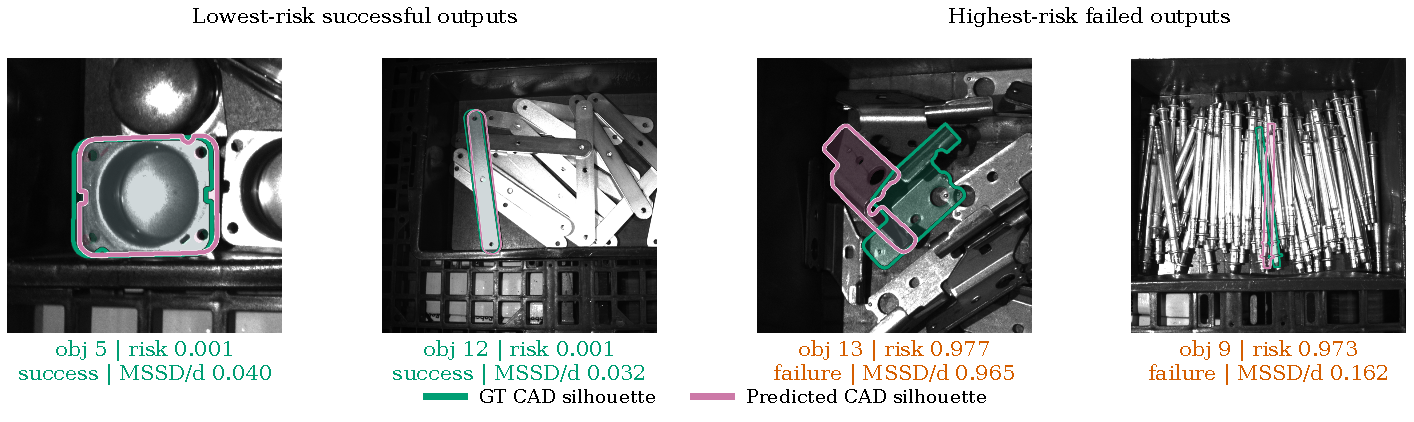
\includegraphics[width=0.98\textwidth]{reports/r2/figures/r2_risk_examples.pdf}
  \caption{Recorded Photoneo outputs at the extremes of the frozen M6-R2 risk ranking: two lowest-risk successes and two highest-risk benchmark failures. Green and magenta contours are ground-truth and predicted CAD silhouettes with contrasting halos. Success uses the sealed joint criterion (normalized MSSD $\leq 0.10$ and MSPD $\leq 10r$), not human visual judgment. Example selection is post-evaluation and does not affect any metric or gate.}
  \label{fig:r2-risk-examples}
\end{figure*}
